\documentclass[crop,tikz]{standalone}
\usepackage{pgfplots}
\pgfplotsset{compat=1.18}
 \begin{document} 
 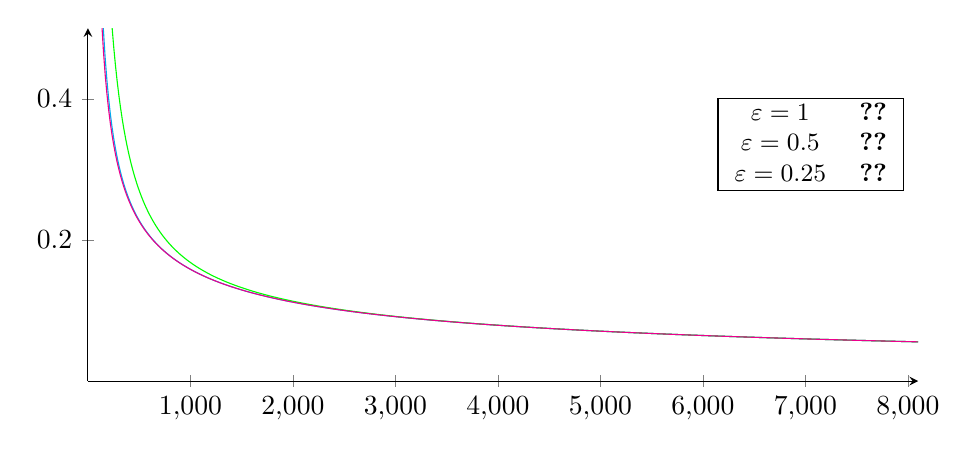
\begin{tikzpicture}
    \begin{axis}[samples=600, width=\textwidth, height = .5\textwidth, axis x line=middle,axis y line=middle,ymin = 0, ymax = 0.5, xmin = 0, xmax = 8100, name=boundary]
        \addplot [domain=1:10000, cyan] {5/sqrt(x) + (4/(sqrt(x)*0.5))*exp(-sqrt(x)*0.5/2) + 16/sqrt(x) * exp(-sqrt(x)/4)}; \label{pgfplots:e5}
        \addplot [domain=1:10000, green] {5/sqrt(x) + (4/(sqrt(x)*0.25))*exp(-sqrt(x)*0.25/2) + 16/sqrt(x) * exp(-sqrt(x)/4)}; \label{pgfplots:e25}
        \addplot [domain=1:10000, magenta] {5/sqrt(x) + (4/(sqrt(x)*1))*exp(-sqrt(x)*1/2) + 16/sqrt(x) * exp(-sqrt(x)/4)}; \label{pgfplots:e1}
    \end{axis}  

    \node[draw,fill=white,inner sep=0pt,above left=0.5em] at (boundary.east) {\small
    \begin{tabular}{cc} 
        \(\varepsilon = 1\) & \ref{pgfplots:e1}\\
        \(\varepsilon = 0.5\) & \ref{pgfplots:e5}\\
        \(\varepsilon = 0.25\) & \ref{pgfplots:e25}\\
    \end{tabular}};
    \end{tikzpicture}
\end{document} 